\chapter{Introduction}
\setheader{Introduction}
This document provides a sketch of the system that is going to be built during the context project multimedia services. The architecture of the syste is defined by the system's high level components. These components are split in to sub components and sub-systems.

\section{Design goals}
The following design goals will be preserved throughout the project:
\begin{itemize}

\item
\textbf{Deployability}
\\
The system will be developed in such a way that we can always deploy the most current version (\gls{ContinuousIntegration} \cite{Duvall}).
Being able to deploy the system at any time allows us to keep the work required for a release managable.
Because the current version should be deployable at anytime, developers are enforced to only alter the system in a non-breaking way.
Another advantage is that smaller releases\footnote{We define \textit{smaller releases} as a relatively small change to the codebase.} imply a lower possibility of introducing bugs.

\item
\textbf{Portability}
\\
The frontend should work on \textit{Evergreen} browsers \footnote{<<The term "evergreen browser" refers to browsers that are automatically upgraded to future versions, rather than being updated by distribution of new versions from the manufacturer, as was the case with older browsers.>> - http://www.techopedia.com/definition/31094/evergreen-browser}.
The backend should run on both Windows and Linux server environments capable running Java software.

\item
\textbf{Simplicity}
\\
The system will be developed with simplicity in mind.
Existing \glspl{library} and \glspl{framework} will be investigated and used if applicable, so we can focus on developing the system rather than the tools required to build the system.
This will keep our codebase relatively small and allows us to focus on the user experience and underlying algorithms rather than reinventing the wheel for the used techniques.
% By using dependencies we do not reduce the overall complexity, in fact, these dependencies will most likely include unused funcitonality and come with a learning curve for the developers.
% ^ Not sure what to do with this line, please take into account with review - JW

\item
\textbf{Object-oriented programming}
\\
\gls{OOP}\cite{Wirfs-Brock} will be used to develop the system.
We will separate the system into subsystems and components (\glspl{Package}, \glspl{Class} and \glspl{Interface}).
This should enable code reuse and extensibility, and improve the testability of the sytem, because each component can be tested individually\cite{Binder}.

\item
\textbf{Usability}
\\
Users should be able to use Moodcat intuitively.
All features of MoodCat should work for modern browsers.
Moodcat should work properly with accessibility tools like screenreaders.

\end{itemize}

\chapter{Software architecture views}
This chapter discusses the architecture of the system.
The system is first decomposed into smaller subsystems and the dependencies between the subsystems are explained.
In the second paragraph the relation between the hardware and software of the system is elaborated.
The third paragraph illustrates the data management of the system.

\section{Subsystem decomposition}
Moodcat is subdivided into two components: the frontend website and the backend processing service.
In this chapter we will explain how these components are composed and how they interact with each other.

\begin{figure}[H]
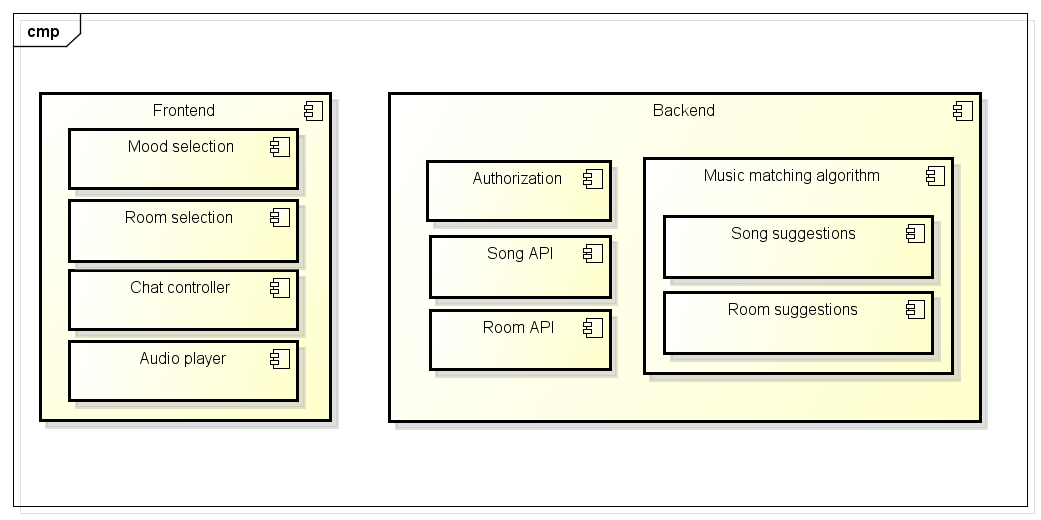
\includegraphics[scale=.6]{architectureOverview.png}
\caption{Architecture overview for Moodcat}
\label{fig:architectureOverview}
\end{figure}

\subsection{Moodcat Frontend}
The frontend will be the visible part for the user.
After logging in to our services, the user will be able to select his mood and based on that MoodCat will provide several music listening rooms.
In these rooms the user can interact with other users through the chat while listening to the music.

\begin{figure}[H]
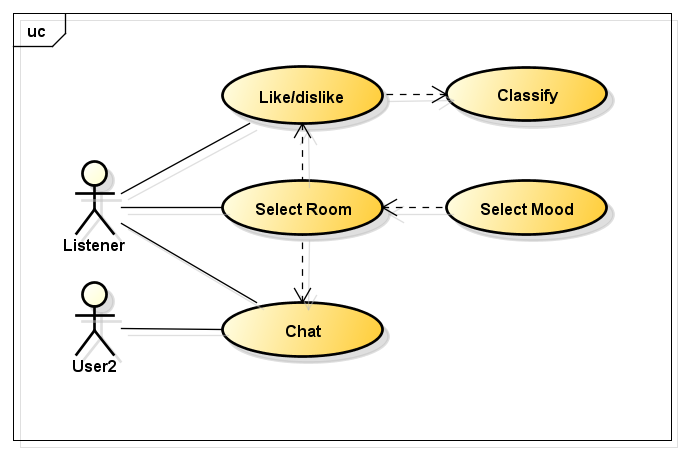
\includegraphics[scale=.4]{useCases.png}
\caption{Use case diagram for Moodcat}
\label{fig:MoodCatUseCase}
\end{figure}

\par
The MoodCat frontend will be web-based.
This allows us to support all modern devices which enables a large target audience.
We will develop the frontend using modern techniques as \Gls{HTML}\cite{HTML}, \Gls{JS} and \Gls{CSS}\cite{CSS}.
Twitter Bootstrap will be used as boilerplate for our own customized CSS theme.

\par
AngularJS\cite{AngularJS} will be used as web framework, providing us two-way data binding between the user interface and backend, and a standardized way of composing user interface controlling logic through \textit{controllers}, \textit{services} and \textit{directives}.

\par
The Object-oriented\cite{Wirfs-Brock} and Dependency Injection\cite{angularDI} driven nature of AngularJS makes it suitable for unit testing\cite{Binder}.
Testing the frontend codebase will be done using the Karma\cite{Karma} testrunner, the Jasmine\cite{Jasmine} testing framework and the PhantomJS\cite{PhantomJS} headless\footnote{JavaScript runs in browsers and the written logic needs a DOM to interact with. A headless browser does not actually render the page and is therefore much faster in intergration tests.} browser.

\label{frontendstructure}
\subsubsection{Frontend structure}
Angular works with \textit{controllers}, \textit{services} and \textit{directives}.
Directives can thought of as physical elements on the webpage, yet they have \textit{controller} logic attached to it.
Directives can be double binded to a scope. This means that the directive can both read and write to the scope.
Scopes in Angular are \glspl{ViewModel}, and can contain both data and methods.
A scope can recursively resolve data from its parent \textit{scope}, this is implemented through JavaScripts \gls{Prototype inheritence}.
The top level scope is the so-called \textit{\$rootScope}.
Services are singleton objects that can be used for shared logic between controllers.

\par
The system will be build around \textit{services} that connect with our backend API, for example the \class{RoomService} that queries rooms and the \class{ChatService} that manages chat messages within a room.
The \textit{\$rootScope} will be used to store data such as the selected moods, current room and the current song.

\subsection{Moodcat Backend}
The Moodcat backend has several subcomponents, each with their own responsibility:
\begin{itemize}
\item the \textit{Static File Server} that serves the frontend website on a webserver;
\item the \textit{SoundCloud integration} which allows for user login and metadata querying.
\item the \textit{REST API} which is used for communication about rooms and songs between the backend and frontend;
\item the \textit{Music Matching Algorithm} which is used to generate music suggestions for rooms and to find a room for a user.
\end{itemize}
In the following paragraphs we will explain the last two subcomponents.

\subsubsection{REST API}
The backend keeps track of which rooms are active and what song is currently played in the room.
When the backed is started, it creates a room instance for each room in the database.
For each room instance, the backend keeps track of a current song, a history of previously played songs 
and a playing queue for future tracks to play.
Rooms, songs and chatmessages all have their own models, which are used to represent their
respective instances that are managed in the backend, and their own entities that are stored in the database.
Splitting up models, instances and entities allows for flexibility in what data is sent to
the frontend and what attributes are stored in the database.
Next to these objects, the REST API uses a nowPlaying model, which is a collection of the time of the song in
a room and the metadata of the song. This nowPlaying model is used for an API endpoint that is more lightweight
than the room model, which makes it more suitable for constant polling so that the frontend can verify
if it's still in sync.

Next to requesting data, the API can process user votes and classifications in order to improve the system.
When an API call results in the change of an attribute of a room, the room is updated in the database.
Furthermore, the backend is responsible for transmitting the chat messages between the users in the room.
An example interaction between the frontend and the backend is given in \ref{fig: backendInteraction}.

\begin{figure}[H]
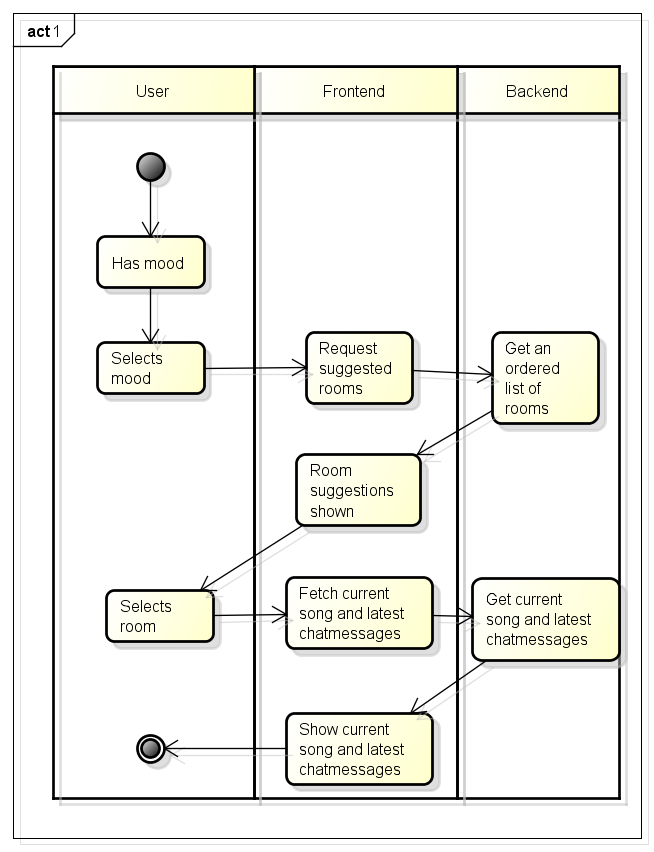
\includegraphics[scale=.4]{backendInteraction.png}
\caption{Example interaction frontend and backend}
\label{fig: backendInteraction}
\end{figure}


\par
The backend and the frontend communicate over \Gls{HTTP} requests in the \Gls{JSON} format.
% We might want to note Websockets at a later point
The REST API will be written in Java using JAX-RS and Jackson.
Jackson serializes Java objects to a JSON string based on their attributes, and vice versa: it is able to deserialize a Java object from a JSON string.
This allows us to use JSON in the frontend, which is ideal in \Gls{JS}, but use classes and objects in Java, which greatly improves the testability of the responses.
The backend will be tested with unit tests written using JUnit and Mockito.

\subsubsection{SoundCloud integration}
Moodcat uses the SoundCloud API for user login, metadata querying and, in the frontend, for streaming.
To keep track of user's points, progress and stats Moodcat lets their users sign in with their SoundCloud account,
when users press the login button they are redirected to the SoundCloud login page, which will, on succesfull login,
provide a SoundCloud user id. This id is used to store and retrieve the statistics of users in our database.

To fill the database with songs we have created a helper program. By default this program uses a list of the 1000 most popular tracks on SoundCloud. We fetch their metadata through the SoundCloud API, extract the relevant data through the object's entities
and store those in the database.

\subsubsection{Music matching algorithm}\label{MatchingAlgorithm}
The music matching algorithm determines and compares moods for songs, rooms and users.
The classification of songs will be done by classification from the user, which will be encouraged with gamification.
Moodcat will improve over time, because the more people classify the more accurate it gets.
All entities are modeled with a valence and arousal vector. Valence and arousal are measured in a range of -1 to 1. By default, a song will be classified with the default vector: valence 0 and arousal 0. This would mean an absolute neutral mood. This classification (mapping) will be updated over time by processing user feedback. Therefore the longer the system is running, the more accurate the classifications become.

When a user votes down, the user will be requested to classify the song.
If there are more up-votes than down-votes the classification will not have effect, because the majority of the audience says the song fits the room.

Using a nearest-neighbour algorithm we will determine which song fits a room and which room fits a user.
This can ultimately be improved by personalising according to the listening history of the user.

\section{Hardware/software mapping}
For navigating through the user interface and posting messages in the chatroom a keyboard and mouse, or a touch screen with onscreen keyboard is required.
We will annotate our elements with proper \Gls{ARIA} accessibilty attributes so that assistive technologies, such as screen readers, will work with our service properly.

\par
Moodcat requires an audio interface to play music.
To interact with the audio interface from the browser, the Web Audio API\cite{WebAudioAPI} and ngAudio\cite{ngAudio} are used.
The users browser should support these technologies in order to use Moodcat.

\section{Persistent data management}
Moodcat has to handle both song data and chatroom data.

\par
We try do deduplicate artists from the Soundcloud data as much as possible. We identify artists in our database by an unique identifier. Besides this identifier, we store the name for the artist. The name will be used to display in the frontend.

\par
For the song we store the basic properties, like artist, song title and duration.
A song has an unique id in our system and also an id from \gls{Soundcloud}, in order to fetch data from Soundcloud.
We also include an url to display the artwork of a song.

Furthermore each song has its own \gls{valence} and \gls{arousal} value, this is updated when users classify the song.
This classification will be done in the Music Matching Algorithm as described above. In order to prevent incorrect or unwanted classifications, we also have to store the netto value of up-votes compared to the down-votes.

\par 
Each room has an unique room identifier, which is used to find the room requested from the API call.
We also store some properties: The name of the room to display on the frontend, the currently playing song including its metadata, 
and a playing queue and history of played songs.
Furthermore, the arousal and valence values of the room are stored.

\par
For a chatmessage we store the author, actual message, timestamp and the room in which the message was posted.

\begin{figure}[H]
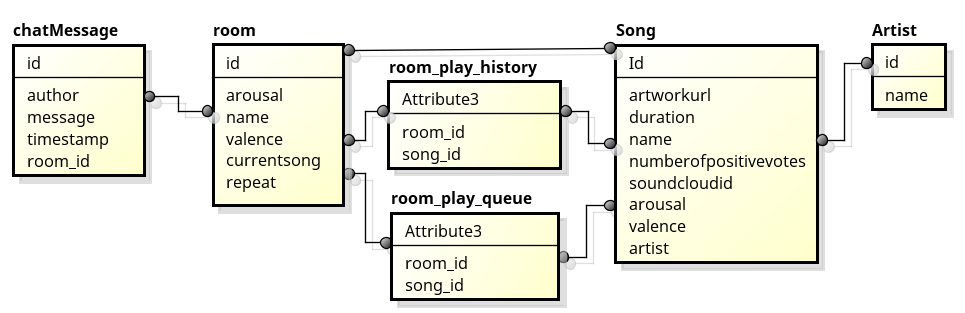
\includegraphics[scale=.6]{erDiagram.png}
\caption{ER diagram for Moodcat}
\label{fig:ER diagram of the described entities}
\end{figure}

\par
Most of the currently used data will be stored in memory, as it would be intensive, for example, to query the database for each chat message that comes in.
However, the data will eventually be persisted in a PostgreSQL\cite{PostgreSQL} \gls{RDB}.
On one hand, it would be impractical to store our entire dataset in memory, on the other hand, then the system can continue where it has left off after a restart.

\par
We will connect our Java backend server to the PostgreSQL database using the Java Persistence API (JPA) and the Postgres JDBC driver.
The Hibernate\cite{HibernateORM} \Gls{ORM} (ORM) framework will be used to map Java class instances to tables.
QueryDSL\cite{QueryDSL} JPAQuery will be used to build \Gls{SQL} queries from Java code.
We have chosen for these techniques because they provide a nice and clean API to bind Java objects to database objects.

\section{Concurrency}
In order to scale up to thousands of connected clients, we should develop with concurrency in mind from the very first start.
Moodcat uses the \gls{Soundcloud} API in order to stream media to the clients.
This means that the audio stream does not have to pass through our servers.
We do however have to handle the various API calls to interact with the backend, for example to play the next song or to broadcast a message in a room.

\par
It is important that these requests do not block each other, therefore we have chosen a servlet container, Jetty, that uses asynchronous sockets - which will not block if there is no data to receive yet.

\par
Besides the communication with the clients, Moodcat should also keep its algorithm (described in \ref{MatchingAlgorithm}) running in the background.
This algorithm will run in seperate threads to optimize throughput.
These seperate threads will get a specific task assigned, which has his local data to compute on.
Deadlocks will be prevented because the spawned threads will be joined before acquiring locks in synchronized statements.
This will happen when we persist the algorithm output in the database.

\section{Scalability}
Concurrent clients are one thing, but we also have to scale the algorithms for growth.
Initially, we planned on a nearest neighbours algorithm to match songs to rooms.
Later on, we found out that (while this works well for small datasets,) finding the nearest neighbours in a system of a few million songs can prove to be a lot harder.
The goal is clear: Find a way for the system to scale further.
We went over several iterations of the system.
Once we realised the issue with plain Nearest Neighbours, we went for an ANN\footnote{Approximate nearest neighbour} algorithm to be able to use the nearest neighbour algorithm.
This initially was planned to be implemented using a \gls{KD-tree}.
However, this would cause memory issues due to a O(N) space complexity of the algorithm.
The second suggestion was retrieving a random subset of songs to run the NN algorithm on.
We ran some calculations, and it looked promising, but it underestimated the locality clustering of the data. 
We also considered \gls{LSH}, but this is better suited for high-dimension data, and MapReduce, but this wasn't feasible for the amount of time we had.
In the end, we threw away the original NN implementation we had and use spatial indexing in the database, using \gls{R-tree}s.

\section{Design Patterns}

Due to the usage of various libraries and frameworks, our codebase does not contain a lot of helper mechanisms.
Therefore the number of design patterns implemented is lower, because we use a lot of patterns defined in the frameworks.

The design patterns we use, as they are defined in the frameworks, are:

\begin{enumerate}
\item Lazy initialization (Hibernate):\\
OneToMany-relations are fetched from the database when they are needed.
This not only makes retrieval of entities that use embeddables faster, we can also database calls.
For example most of the time we are not interested in the songs that an artist produced, just his/her name.

\item Object pooling (RestEasy, Guice):\\
The http-connection to SoundCloud and database-connection to our PostgreSQL database are pooled for re-use.
This way we only have to set up the connection once using said frameworks and reduce object retrieval time.
The \class{SoundCloudAPIConnector} uses a RestEasyClient.
The database connection is handled by C3PO which is an extension of Hibernate, our \gls{ORM} framework.

\item Memento (JPA, Guice):\\
All database updates and retrievals are transactions, which implement the Memento design pattern.
This makes sure that all database changes are ACID\cite{ACID}.
Classes instantiated through Guice dependency injection can annotate methods with @Transactional, so that the method is intercepted to enforce that the method is ran in a database transaction.
This starts a new transaction if no transaction is active for the current thread.
If any exceptions occur (either in the Java or database layer - for example unmet key constraints) the transaction will automatically be rolled back after the exception has been propagated upwards.
All extensions of \class{AbstractDAO} have transactions.

\item Builder (QueryDSL, HttpClient):\\
We use QueryDSL in order to easily create SQL queries that map to our Hibernate entities.
QueryDSL allows you to write SQL queries using a builder pattern.
For each database entity, QueryDSL generates a few classes (so named QClasses) which allow you to write SQL queries using a builder pattern.
This introduces type safety, because schema changes will now cause compile errors if a query is not updated.

The HttpClient that we use for our HTTP calls to the SoundCloud API also uses a builder pattern to set the path, parameters and headers for the request to be made.

\end{enumerate}

The design patterns we implemented ourselves are:

\begin{enumerate}
\item Singleton:\\
In order to enforce a single controlling unit, all of our backends \cite{backend} are singleton.
For example the \class{ChatBackend} contains all \class{RoomInstances}, which should be stateful\footnote{Stateful room instances should not be confused with the stateless nature of the REST-api. From the clients point-of-view all requests are stateless and don't influence future requests.} in order to maintain cached collections of \class{ChatMessages}.
This speeds up message retrieval for users that join a room.
It also reduces the amount of database updates, which lowers the network traffic.
Also, the Angular \textit{services} for the backend, described in \ref{frontendstructure}, follow the singleton pattern as well.

\item Facade:\\
All APIs and backends implement the Facade design pattern.
They are a single end-point which can connect several backends or DAOs.
Therefore we can change the actual storage- and retrieval-structure, while making sure our API end-points and backends still provide the correct data in the correct structure.

\item Observer (not implemented yet):\\
We will use the Observer pattern after converting our currently poll-based architecture to a stream pipeline using websockets.
This way the frontend can continuously receive updates whenever the backend notifies the clients.
Therefore chat messages can be instantly received and no unnecessary calls shall be made to the frontend.
Currently the frontend polls every second the backend to check if there are updates.
\end{enumerate}
